\section{くりくり$\heartsuit$びぶんにゅうもん♪}
\subsection{微分のイントロダクション}
\ \\
\kao{fig/holmy.png}{それでは微分について学んでいきます。}\\
\kao{fig/rosia.png}{微分ってあれでしょ、ドラマでよく頭良さそうな人がやってる如何にも理系~な感じのやつでしょ?}\\
\kao{fig/jacklyn.png}{黒板に難しい数式がビッシリ書いてあるやつやな~}\\
\kao{fig/tsukino.png}{とっても難しそうなの…}\\
\kaot{fig/holmy.png}{そうですね…多分全然馴染みのない概念だと思いますので、まず簡単な具体例を考えてみましょう。\\
物体を地点$y_0$から落下させることを考えます。そのときの地上からの高さは時間$t$に対して
\[
    y(t)=y_0-\frac{1}{2}gt^2\ \ (g\mbox{は定数})
\]
となることが実験的に分かってます。グラフを描くと以下のようになります。}\\
\[
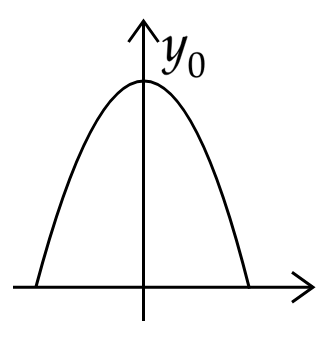
\includegraphics[width=4cm]{fig/2_0_gfunc.png}
\]
\kao{fig/jacklyn.png}{理科の実験とかであるやつやな~}\\
\kaot{fig/holmy.png}{この$y$について、時間$t_1$での速度を求めてみましょう。ただし$y(t_1)>0$です。
速度を求めるために次のように考えてみます。小学校の計算では
\[
    \mbox{(距離)}=\mbox{(速度)}\times\mbox{(時間)}
\]
だったので速度$\bar{v}$は$t_1$秒から$h$秒後の変化に、どれくらい移動するかの割合(変化率)として考えてみます。}
\kaot{fig/holmy.png}{つまり、式で書くと
\begin{align*}
    \bar{v}h &= y(t_1+h) - y(t_1) = -(y_0-y_0) - \frac{1}{2}g(t_1+h)^2 + \frac{1}{2}gt_1^2\\
    &= -\frac{1}{2}g(t_1^2+2t_1h+h^2-t_1^2) = -\frac{1}{2}g(2t_1h+h^2)
\end{align*}
よって
\[
    \bar{v} = -g(t_1+\frac{1}{2}h)
\]
と考えます。これを$t_1$秒から$t_1+h$秒の{\bf 平均速度}といいます。\\
これは、$y(t_1)$と$y(t_1+h)$のグラフの点を結んだ直線の傾きになってます。} \\
\[
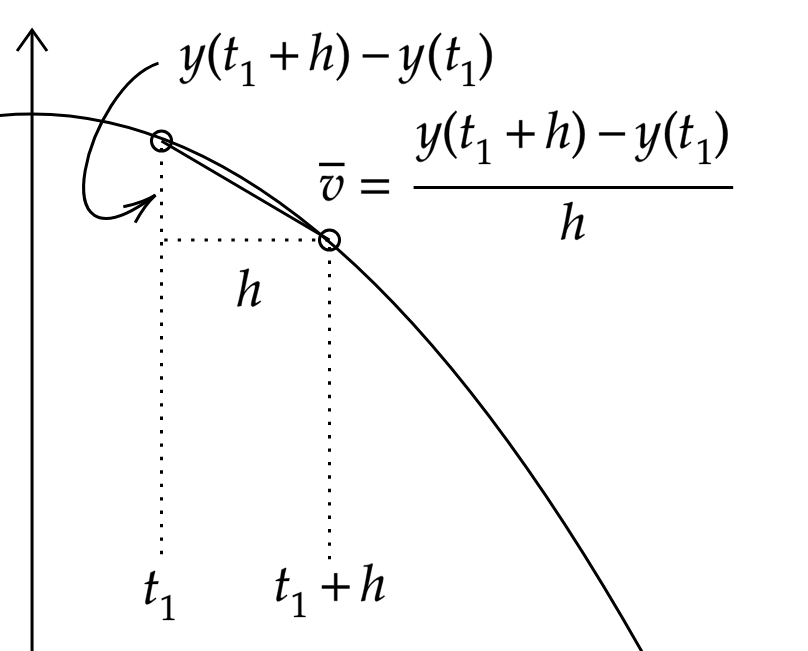
\includegraphics[width=6cm]{fig/2_0_g_ave_speed.png}
\]
\kaot{fig/rosia.png}{たしかにこれで$t_1$から$t_1+h$の地面からの位置は求められそうだけど、$t_1$から$t_1+h$からの間は速度は変わり続けているからズレが生じるんじゃない?\\
距離$=$速度$\times$時間の式みたいに単純に距離が求められないから速度としては不十分じゃないかしら?}\\
\kaot{fig/holmy.png}{その通りです、平均速度はあくまである区間での平均した速度となっているため、区間内の変化を捉えることができません。\\
そこで、$h$を非常に小さくした{\bf 瞬間速度}を考えます。今、$t_1$から$t_1+h$の平均速度$\bar{v}$が
\[
    \bar{v} = -g(t_1+\frac{1}{2}h) = -gt_1-\frac{1}{2}gh
\]
でしたが、$h$が非常に小さいので、第2項の$\frac{1}{2}gh$は0に近づくので、瞬間速度$v$は
\[
    v = -gt_1
\]
となります。ここで、$h$を0に近付けたときに$\bar{v}$が$-gt_1$に近づくということを
\[
    \lim_{h\to 0}\bar{v} = -gt_1
\]
または
\[
    \bar{v} \to -gt_1\ \ (h\to 0)
\]
と書き、$\bar{v}$の{\bf 極限}といいます。}\\
\[
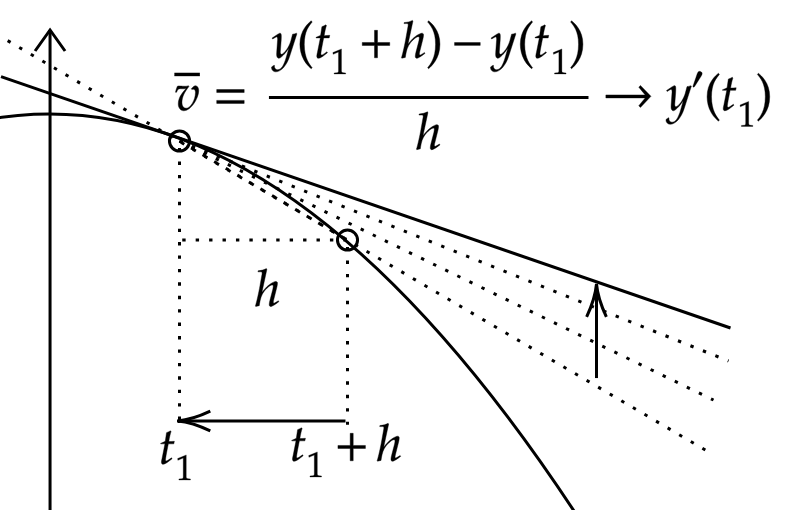
\includegraphics[width=6cm]{fig/2_0_g_diff.png}
\]
\kao{fig/jacklyn.png}{言われてみるとそうなりそうやなぁ}\\
\kaot{fig/holmy.png}{ここで、平均速度$t_1$から$t_1+h$の点を結ぶ直線の傾きとして見れましたが瞬間速度は$t_1$の点における接戦の傾きになっています。\\
さて、この瞬間速度を求めた方法をどんな関数$f(x)$にも適用することを考えます。関数$f(x)$の$x=a$から$x=a+h$での平均変化率を求めると
\[
    \frac{f(a+h)-f(a)}{h}
\]
となります。}\\
\kaot{fig/holmy.png}{ここで、$h$を限りなく0に近付けた
\[
    \lim_{h\to 0}\frac{f(a+h)-f(a)}{h}
\]
の値が存在すれば、それを$f(x)$の$x=a$における{\bf 瞬間変化率}、{\bf 導値}、{\bf 微分係数}と言い、この値を求めることを{\bf 微分}するといいます。
$f$の$x=a$における微分係数を$f^\prime(a),\frac{d}{dx}f(a)$など書きます。微分係数は{\bf 瞬間速度}と同じように、その点での接線の傾きとなっています。\\
$f$に対して微分係数が定義できる点から微分係数を対応させた関数として見ることができ、これを{\bf 導関数}といいます。
導関数の値は各点での傾きとなるので、0となることで平らとなり、周りの値よりか高いか低いかが分かります。これが微分と最大最小との関係を示唆する意味となっております。}\\
\kao{fig/jacklyn.png}{坂を上ってるときに、傾きが緩くなったらもしかしたら頂上かもって錯覚する感じやな!}
\kao{fig/tsukino.png}{限りなく0に近い数…想像つかないの…}\\
\kaot{fig/holmy.png}{そうですね、ツキノの言う通り、限りなく0に近づくという操作が非常に曖昧であり、数学では極限という概念は18世紀に誕生したものですが、19世紀ではその定義を巡って物議をかもしました。\\
そして、この単純な極限の定義(無限小式)は見直されて厳密な定義($\varepsilon\delta$式)が与えられました。
しかし、20世紀になり、数学が発展すると旧来の定義も$\varepsilon\delta$式も同じであることが証明されました。\footnotemark[1]}
\footnotetext[1]{17世紀、フェルマーやデカルトによって関数の接線を求める研究がされ、ニュートン、ライプニッツによって微分という手法は定式化された。そして極限の取り扱い($\varepsilon\delta$論法)、実数の性質を見直し厳密に定めたのはコーシー、ワイエルシュトラス、デデキントらの19世紀の数学者であった。
そして、20世紀、ロビンソンによって数学基礎論を用いて、それまでの$\varepsilon\delta$論法と旧来の無限小解析が両立する超準解析が構成された。\\
参考: ブルバキ,数学史}\\
\kao{fig/rosia.png}{ふーん、微分って昔からあるのね。}
\kaot{fig/holmy.png}{そうですね、200年前からありますが、微分は数学の歴史上大きな影響を与えたのは確かです。定義だとわかりづらいので、単純な定義で、具体例を計算してみましょう。}\\
\paragraph{例: 微分を計算してみよう}\ \\
\kao{fig/holmy.png}{では、次の関数を微分してみましょう。}
\begin{enumerate}[$(1)$]
\item $f(x)=C$\ \ ($C$:定数)について$f^\prime(x_0)$
\item $f(x)=x^n$について$f^\prime(x_0)$
\item $f(x)=|x|$について$f^\prime(0)$
\end{enumerate}
(1) \\
\kao{fig/holmy.png}{まずは(1)ですが、これは簡単なので、計算してみてください。}\\
\kao{fig/jacklyn.png}{やってみるで~ええと、微分の定義の通り計算すると…
\[
    f^\prime(x_0) = \lim_{h\to 0} \frac{f(x_0+h)-f(x_0)}{h} = \lim_{h\to 0}\frac{C-C}{h} = 0
\]
やな!}
\kao{fig/rosia.png}{0になっちゃったわね。}\\
\kao{fig/holmy.png}{そうですね、この関数を見てみると、とくに値が変化せずに一定の値なので、変化率は0となります。よってどんな点の微分係数も0となります。}\\
(2)\\
\kaot{fig/holmy.png}{続いて(2)を解きますが、これを解く前に次の命題を示しましょう}\\
\begin{breakbox}
    \begin{Prop}
        \label{Prop2_0_1}
        任意の実数$a,b$について$n\geq 2$について
        \[
            (a+b)^n = a^n + na^{n-1}b + R^{(n-2)}(a,b)
        \]
        ただし、$R^{(n-2)}(a,b)$は
        \[
            R^{(n-2)}(a,b) = \sum_{i=0}^{n-2} c_i^{(n-2)}g(b)a^i
        \]
        と書け、$b^2|R^{(n-2)}(a,b)$となる。\footnotemark[1]
    \end{Prop}
\end{breakbox}
\ \\
\kao{fig/tsukino.png}{なんか変な記号でたの、$b^2|R^{(n-2)}(a,b)$ってなんなのなの?}\\
\kao{fig/holmy.png}{これは割り切るといって$p|q$は$q=pr$となるような$r$が存在することを言います。\footnotemark[2]}
\footnotetext[1]{一般に$\sum_{i=0}^{n}c_iX^i, c_i\in \mathbb{R}$となる式を$n$次の$X$について多項式といい、その集合を$\mathbb{R}[X]$とかく、また各$c_iX^i$を単項式という。とくに$R^{(n-2)}(a,b)$は2変数多項式で$\in \mathbb{R}[a,b]$である。}
\footnotetext[2]{前作「ろーほるすーがくれっすん」(\url{https://irisu-in-wonderland.tumblr.com/post/156533872627})にも同様の記号が登場するが、前作は整数$\mathbb{Z}$の範囲だった。\\
今回の$b^2|R^{(n-2)}(a,b)$は$\mathbb{R}[a,b]$で考えてる。このように整数と多項式の間で足し算と掛け算のみに着目すれば同じことを考えられる。掛け算と足し算が定められ、全ての元に逆数が存在するとは限らない構造を{\bf 環}という。}\\
\begin{proof}
    $n=2$のとき、
    \[
        (a+b)^2 = a^2+2ab+b^2
    \]
    となり、$R^{(0)}(a,b)=b^2$とすれば主張は正しい。\\
    $n-1$のときに成立するとして、$n$のとき
    \begin{align*}
        (a+b)^n &= (a+b)^{n-1}(a+b) = (a^{n-1}+(n-1)a^{n-2}b+R^{(n-3)}(a,b))(a+b)\\
        &= (a^n+(n-1)a^{n-1}b+aR^{(n-3)}(a,b))+(a^{n-1}b+(n-1)a^{n-2}b^2+bR^{(n-3)}(a,b))\\
        &= a^n + na^{n-1}b + (aR^{(n-3)}(a,b) + (n-1)a^{n-2}b^2 + bR^{(n-3)}(a,b))
    \end{align*}
    となる。ここで$R^{(n-2)}(a,b) = aR^{(n-3)}(a,b) + (n-1)a^{n-2}b^2 + bR^{(n-3)}(a,b)$とすれば、$aR^{(n-3)}(a,b)=\sum_{i=0}^{n-3} c_i^{(n-3)}g(b)a^{i+1}$であり、$a$のべき乗の数は$n-2$を超えない。
    また、$b^2|aR^{(n-3)}(a,b),b^2|(n-1)a^{n-2}b^2,b^2|bR^{(n-3)}(a,b)$なので$b^2|R^{(n-2)}(a,b)$となる。よって、示された。
\end{proof}
\ \\
\kao{fig/tsukino.png}{なんか不思議な証明なの。}\\
\kao{fig/holmy.png}{このように$n$までの式で一番最初(今回の場合は$n=2$)を示し、$n-1$を示したあとに$n$を示す証明法を{\bf 数学的帰納法}といいます。このように証明すればどんな自然数の$n$にも証明することができます。}\\
\kao{fig/rosia.png}{ええっと、前に教えてもらったっけ?}\\
\kaot{fig/holmy.png}{そうですね…私もうろ覚えですが教えた気がします…\footnotemark[3]\\
では、準備がそろいましたので、$x^n$の微分をしてみましょう。まず$n=1$の場合です。これは簡単で
\[
    f^\prime(x_0) = \lim_{h\to 0} \frac{f(x_0+h)-f(x_0)}{h} = \lim_{h\to 0}\frac{x_0+h-x_0}{h} = 1
\]
となります。続いて$n\geq 2$の場合はどうなるかというと…
\[
    f^\prime(x_0) = \lim_{h\to 0} \frac{f(x_0+h)-f(x_0)}{h} = \lim_{h\to 0}\frac{(x_0+h)^n-x_0^n}{h}
\]
ここで$(x_0+h)^n$に\ref{Prop2_0_1}を用いて
\begin{align*}
    \lim_{h\to 0}\frac{(x_0+h)^n-x_0^n}{h} &= \lim_{h\to 0}\frac{(x_0^n+nx_0^{n-1}h+R^{(n-2)}(x_0,h))-x_0^n}{h} \\
    &= \lim_{h\to 0}\frac{nx_0^{n-1}h+R^{(n-2)}(x_0,h)}{h} \\
    &= \lim_{h\to 0}\left( nx_0^{n-1} + \frac{R^{(n-2)}(x_0,h)}{h} \right)
\end{align*}
となります。今、$R^{(n-2)}(x_0,h)=h^2Q(x_0,h)$と表せるので、
\[
    \lim_{h\to 0} \frac{R^{(n-2)}(x_0,h)}{h} = \lim_{h\to 0} h Q(x_0,h) = 0
\]
となり、よって
\[
    f^\prime(x_0) = nx_0^{n-1}
\]
が証明されました。}
\footnotetext[3]{「ろーほるすーがくれっすん」(\url{https://irisu-in-wonderland.tumblr.com/post/156533872627})の付録A参照}\\
\kao{fig/rosia.png}{とっても盛沢山ね…}\\
\kao{fig/jacklyn.png}{せやなぁ~計算複雑やったわ~}\\
\kao{fig/holmy.png}{実は命題\ref{Prop2_0_1}は厳密には
\[
    (a+b)^n = _nC_0 a^n + _nC_1 a^{n-1}b + _nC_2 a^{n-2}b^2 \cdots + _nC_{n-1}ab^{n-1}+_nC_n b^{n}
\]
とかけます。ここで$_nC_r$は
\[
    _nC_0 = 1, _nC_n = 1, _nC_r=\frac{n\cdot (n-1)\cdots (n-r+1)}{r\cdot (r-1)\cdots 1}
\]
です。}\\
\kao{fig/jacklyn.png}{あ、なんか教科書でみたことあるかもしれんなぁ~}\\
(3)\\
\kao{fig/holmy.png}{あと、もう少しの辛抱ですよ! 最後の問題を解いてみましょう。}\\
\kao{fig/rosia.png}{$f(x)=|x|$の$f^\prime(0)$を求めるんだよね? 
でも、$f(x)=|x|$って$x>0$のとき$f(x)=x$だから、(2)から$f^\prime(0)=1$なんじゃないの?}\\
\kaot{fig/holmy.png}{たしかにそう考えられます。しかし、次のようにも考えられます。$x<0$のとき$f(x)=-x$だから$x<0$から近付けたらその微分係数は$f^\prime(0)=-1$になりませんか?}\\
\kao{fig/rosia.png}{言われてみればそうね…どっちが正しいんだろ…}\\
\kaot{fig/holmy.png}{このように、極限が近づく向きによって答えが変わるケースがあります。特に近づく方向を明示するために$x$が$a$に$a<x$から近づく場合は
\[
    \lim_{x\to a+0} f(x), \lim_{x\to a,x>a} f(x)
\]
などと書きます。最初にロージアが考えたのがこちらですね。\\
また、$x$が$a$に$a<x$から近づく場合は
\[
    \lim_{x\to a-0} f(x), \lim_{x\to a,x<a} f(x)
\]
と書きます。}\\
\kao{fig/tsukino.png}{結構ややこしいの…これって結局どっちが正しいの?}\\
\kaot{fig/holmy.png}{実は、どっちも正しいです。$x\to a$は$x\to a+0$と$x\to a-0$の値が等しい時のみ定義されます。つまり
\[
    \lim_{x\to a}f(x) = \lim_{x\to a,x<a} f(x) = \lim_{x\to a,x>a} f(x)
\]
となります。逆に異なる場合は極限を定義できないことになります。\\
つまり、この問題は
\[
    \lim_{h\to 0, h>0} \frac{f(h)-f(0)}{h} = 1, \lim_{h\to 0, h<0} \frac{f(h)-f(0)}{h} = -1
\]
となり、極限は存在しないことになります。}\\
\kao{fig/jacklyn.png}{へ~極限が存在しないんやなぁ~そんなんあるんやな!}\\
\kao{fig/rosia.png}{解答が存在しないってなんか反則じゃない?}\\
\kao{fig/holmy.png}{いえ、数学の世界では存在しないことを証明することはよくありますよ?}\\
\kao{fig/jacklyn.png}{せやで~目潰しも金的もありのバリトゥードの世界なんやで?}\\
\kao{fig/tsukino.png}{ヤってやるなの~}\\
\kao{fig/holmy.png}{バリトゥードて…}
\dotfill \hspace{6cm}\\
\ \\
\paragraph{例: 微分で関数の大まかな形を見てみよう}\ \\
\kaot{fig/holmy.png}{先ほど、微分を使えば関数がどこで平らになるか、どこで傾いてるかがわかるといいました。関数を微分することで関数の大まかな形(概形)をみることができます。\\
たとえば$y=(x-a)(x-b)^2$を考えてみましょう。}\\
% TODO: 図
\kao{fig/rosia.png}{これってたしか$x=a,x=b$で0になるような二次関数よね。}\\
\kaot{fig/holmy.png}{そうですね。では、導関数を求めることでその形になることが大まかにわかることを見ていきます。$y=(x-a)(x-b)^2$を展開すると
\[
    (x-a)(x-b)^2 = x^2-(a+b)x+ab
\]
となります。実は、関数の微分は各項の微分となることが分かってます\footnotemark[1]。つまり、
\[
    (x^2-(a+b)x+ab)^\prime = (x^2)^\prime-((a+b)x)^\prime+(ab)^\prime
\]
よって、先ほどの例から
\[
    (x^2-(a+b)x+ab)^\prime = 2x-(a+b)
\]
となります。}
\footnotetext[1]{
    関数$f,g$について$(f(x)+g(x))^\prime=f(x)^\prime+g(x)^\prime$となる。これは\S 2.2.1で示す。
}\\
\kao{fig/tsukino.png}{これが$y=(x-a)(x-b)$のかたちになってるの…?}\\
\kaot{fig/holmy.png}{一見わからないですが、導関数を見ていきましょう。導関数$y^\prime = 2x-(a+b)$は$x=\frac{a+b}{2}$で0になり、その前後で$-$から$+$に代わってます。
\[
    \begin{tabular}{|l||l|l|l|l|l|} \hline
        $x$ & $-\infty$ & $x < \frac{a+b}{2}$ & $x=\frac{a+b}{2}$ & $\frac{a+b}{2} < x$ & $\infty$ \\ \hline\hline
        $y^\prime$ & $-\infty$ & $-$ & 0 & $+$ & $\infty$ \\ \hline
    \end{tabular}
\]
つまり、傾きが$x=\frac{a+b}{2}$より左では左斜め下で、$x=\frac{a+b}{2}$で平らになり、より右にいくと右上に上がるようになっています。
さらに$+$に行けば行くほど$y^\prime$の値は大きくなり$-$に行けば行くほど小さくなるので$|x|$の値が大きくなるほど傾きは急になっていきます。}\\
\[
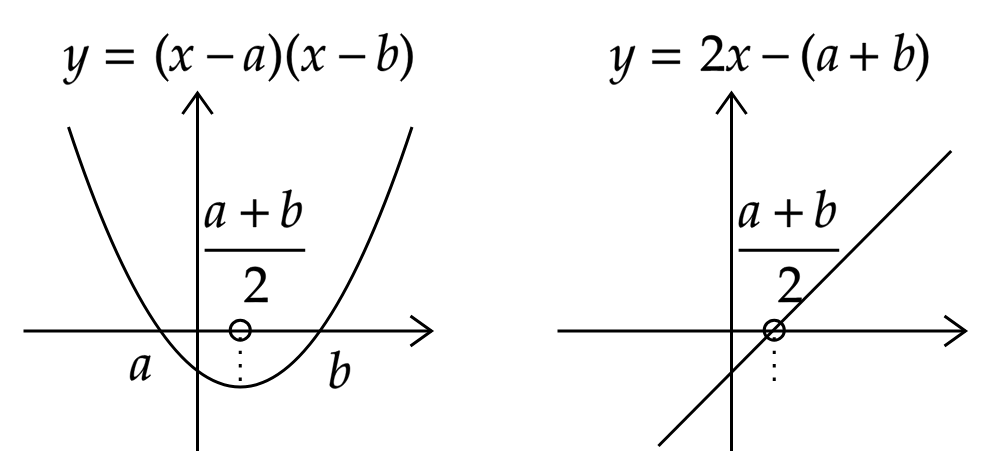
\includegraphics[width=8cm]{fig/2_0_minmax.png}
\]
\kao{fig/jacklyn.png}{こういう感じで微分を使えば関数の形が分かるんやね~}\\
\kao{fig/holmy.png}{そうですね、二次関数だけでなく、三次関数、四次関数、さらに一般の関数についてもその大まかな形がわかります。}
\dotfill \hspace{6cm}\\
\ \\
\kao{fig/holmy.png}{例を見てわかる通り、微分を計算するのに極限について、厳密に考える必要があります。極限とは何なのか、さらには実数とは何なのかについて考えて行きましょう!}
\newpage